\documentclass[../main.tex]{subfiles}
 
\begin{document}

\section{Eszköz (elektronikai és beágyazott szoftverének) tervezése és összeállítása}
    \subsection{Elektronikai tervezés}
        Az elektronikai tervezést 3 fázisra és az utolsó fázis hibáinak kijavítására bontanám le. Az első fázis első lépései között szerepelt az Ebay-ről vásárolt eszközök tesztelése: működik-e mindegyik, programozható-e a fejlesztői lap, konfigurálható-e a Wifi modul, stb\ldots
        
        Második lépésként megnéztem a mikrovezérlőm lábkiosztását (Abra \ref{fig:stm32f103_pinout}) és az alapján kiválasztottam melyeket fogom használni. 
        
        % https://os.mbed.com/users/hudakz/code/STM32F103C8T6_Hello/wiki/Homepage
        \begin{figure}[h!]
            \centering
            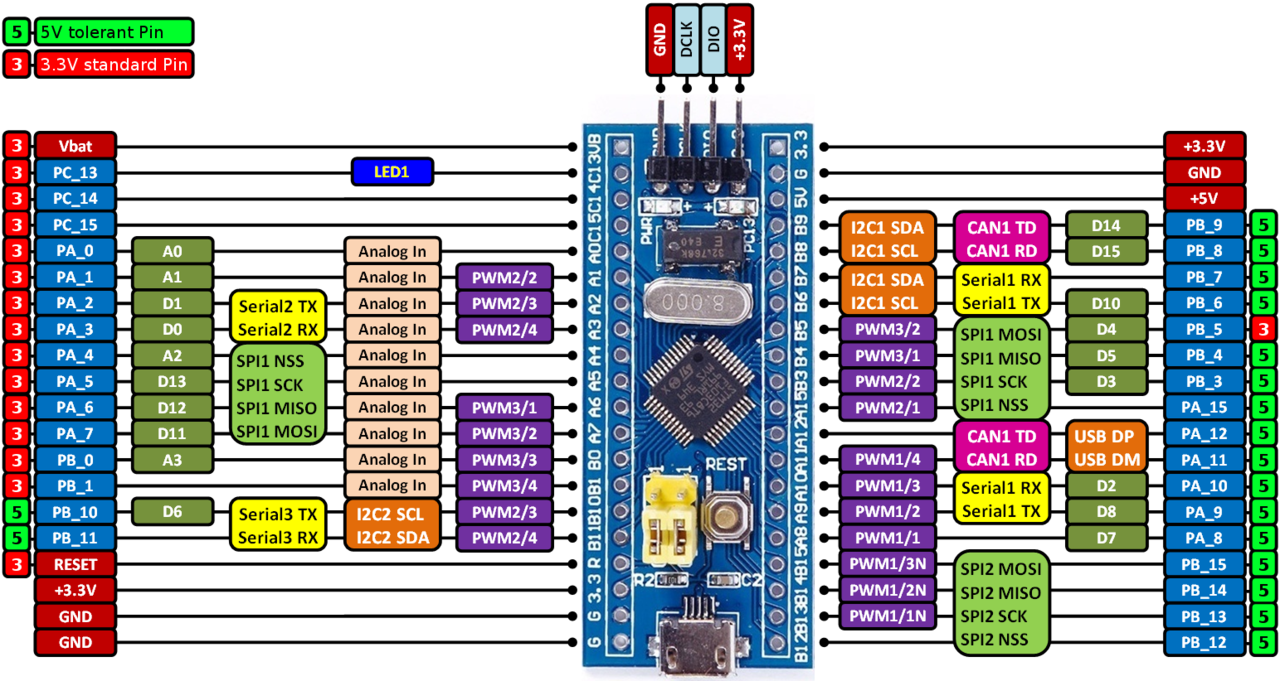
\includegraphics[width=14cm]{resources/pcb_res/stm32f103c8t6_pinout.png}
            \caption{STM32F103C8T6 fejlesztői lap pinout-ja}
            \label{fig:stm32f103_pinout}
        \end{figure}
        
        A PB\_0-s lábat választottam a LED sor vezérlő lábnak, és a PA\_9, PA\_10 (TX,RX) lábakat pedig Wifi modullal kommunikáló UART lábaknak. Minden modulra a megfelelő tápfeszültséget kötöttem, illetve az összes földpotenciált összehuzalosztam, ezátal egy közös földpontot létrehozva. A ESP-01-s modul pinoutja (Ábra \ref{fig:eps01_pinout}) alapján UART lábkat is összekötöttem a megfelelő módon: a mikrovezérlő RX lábát (PA\_10) a Wifi modul U0TXD lábával és mikrovezérlő TX lábát (PA\_9) a Wifi modul U0RXD lábával. 
        
        \begin{figure}[h!]
            \centering
                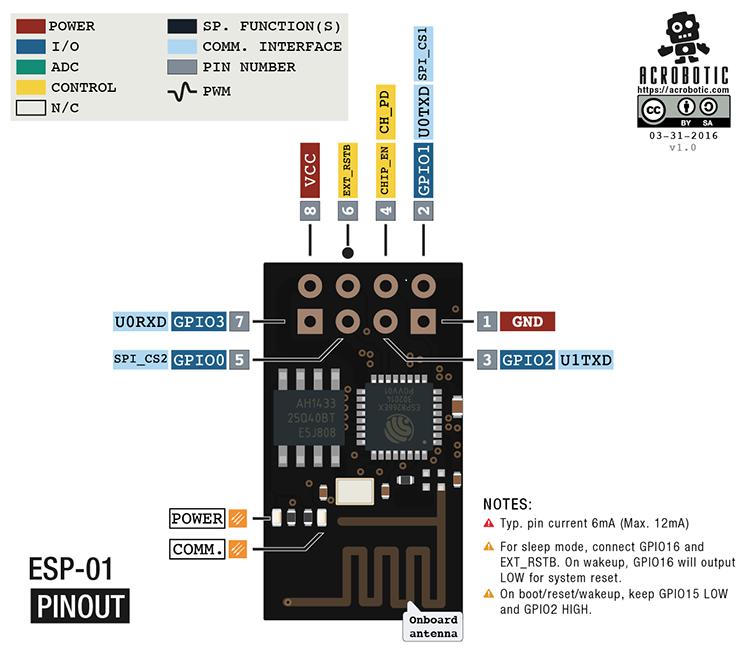
\includegraphics[width=10cm]{resources/pcb_res/esp8266_esp01_pinout.png}
            \caption{ESP-01 pinout-ja}
            \label{fig:eps01_pinout}
        \end{figure}
        
        A WS2811-es IC adatlapján a logikai jelszintes részt áttanulmányozva megállapítottam, hogy a mikrovezérlő 3,3V-os vezérlő jelét még éppen tolerálja a LED sor vezérlő IC 5V-os bemeneti lába (3,2V-os jel igaznak felel meg). 
        
        Ezek alapján összeállítottam a kapcsolást breadboard-on, és az internetről letöltött mintaprogramokat kicsit módosítva elértem, hogy külön-külön működött a Wifi modullal lévő kommunikáció, illetve a LED soron meg tudtam jeleníteni egy fehér színt. Az összeállítással több problémai is volt: a tesztelés során a breadboardból gyakran kicsúsztak a kábelek, a csatlakozások kontaktosak voltak, hamis színeket okozva ezzel a LED soron. 
        
        A problémák orvoslásaként került sor a második fázis kivitelezésére. A Mikrovezérlők c. tantárgy keretében megtanultunk az Autodesk Eagle nevű nyáktervező program használatát. Az internetről letöltöttem és beimportáltam az STM32F103C8T6 mikrovezérlő fejlesztői lapjának
        % https://os.mbed.com/users/hudakz/code/STM32F103C8T6_Hello/wiki/Homepage
        , az ESP8266-os modul ESP-01-es 
        % forras esp libraryra
        típusának a könyvtárait. Létrehoztam egy saját könyvtárt is az Ebay-ről rendelt DC/DC modulnak. Ez a feszültségátalakító állítja elő a 12V-os tápfeszültségből a 3,3V-osat. Egy pár csatlakozó, állatpotjelző LED és ellenállás hozzáadása után összehuzaloztam a megfelelő elemeket. 
        
        \begin{figure}[h!]
            \centering
                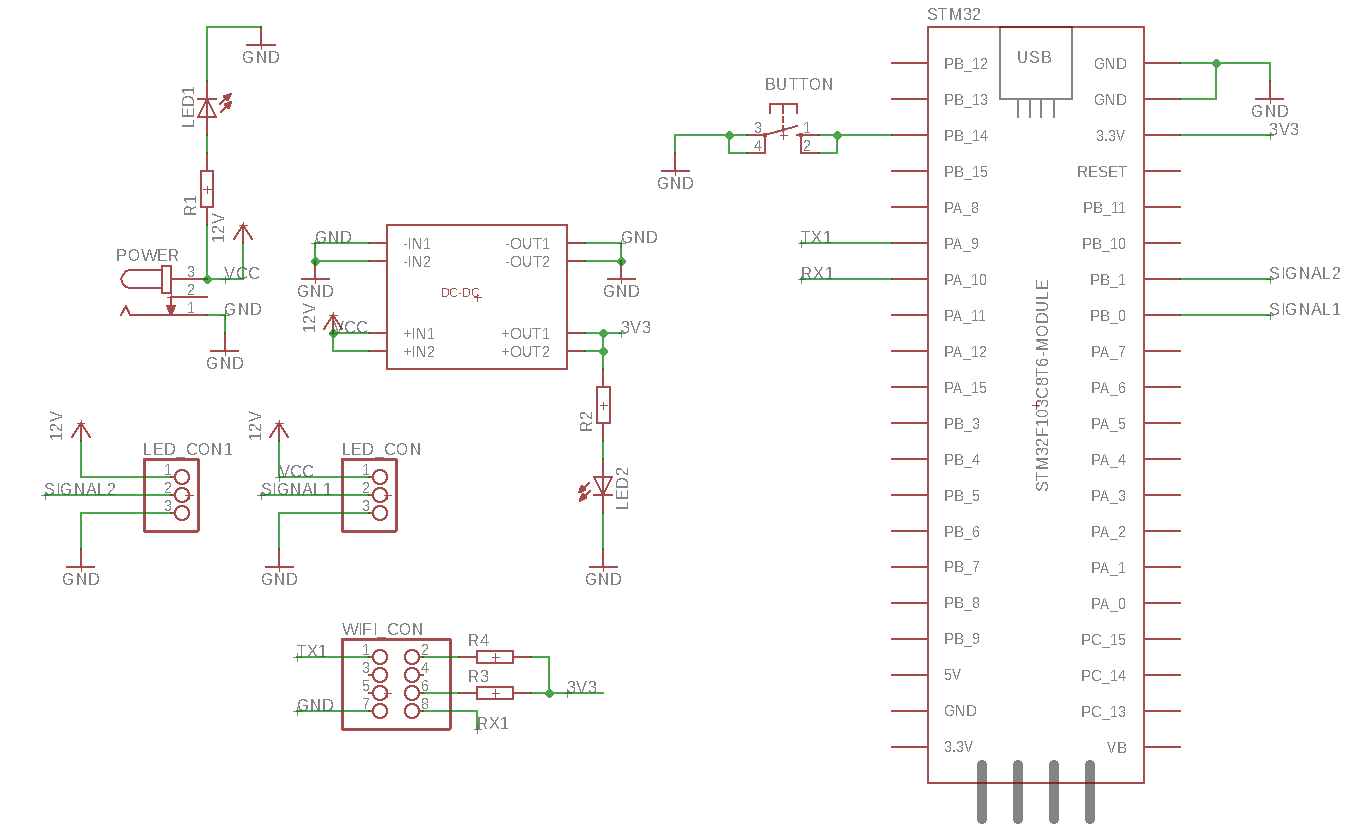
\includegraphics[width=15cm]{resources/pcb_res/schematic_v01.png}
            \caption{2. fázisú kapcsolási rajz}
            \label{fig:schematic_v01}
        \end{figure}
        
        Az elkészült kapcsolási rajz (Ábra \ref{fig:schematic_v01}) után elhelyeztem és összekötöttem az az alkatrészeket az NYÁK-on. Ezen a verzión bekötésre került egy extra gomb (BUTTON) és egy extra csatlakozó (LED\_CON1), hogy mostmár 2 LED sort legyen képes vezérleni az eszköz párhuzamosan. \ref{fig:board_v01}. Ábra szemléltei az így összehuzalozott NYÁK-ot.
        
        \begin{figure}[h!]
            \centering
                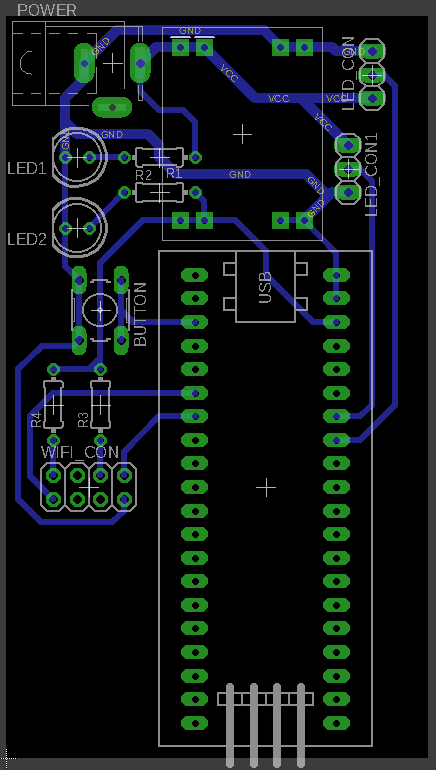
\includegraphics[width=6cm]{resources/pcb_res/board_v01.png}
            \caption{2. fázisú NYÁK-terv}
            \label{fig:board_v01}
        \end{figure}
        
        A NYÁK-ot vasalásos technikával elkészítettem: a tervet fényes papírra lézernyomtatóval kinyomtattam, egy egyoldalas NYÁK-lapra ráhelyeztem, a tonerport vasalóval átvittem a réz felületre, a tonerral nem fedett réz részeket pedig a maratószer lemarattam, és végül acetonnal eltávolítottam, hogy a megmaradt rézfelületre lehessen forrasztani. Az így elkészült NYÁK-ot (Ábra \ref{fig:pcb_v10}) beforrasztottam és az alkatrészeket belehelyeztem. Ezzel a NYÁK-al már el lehetett kezdeni a beágyazott szoftver fejlesztését, az elektronikai rész stabilan működött.
        
        \begin{figure}[h!]
            \centering
                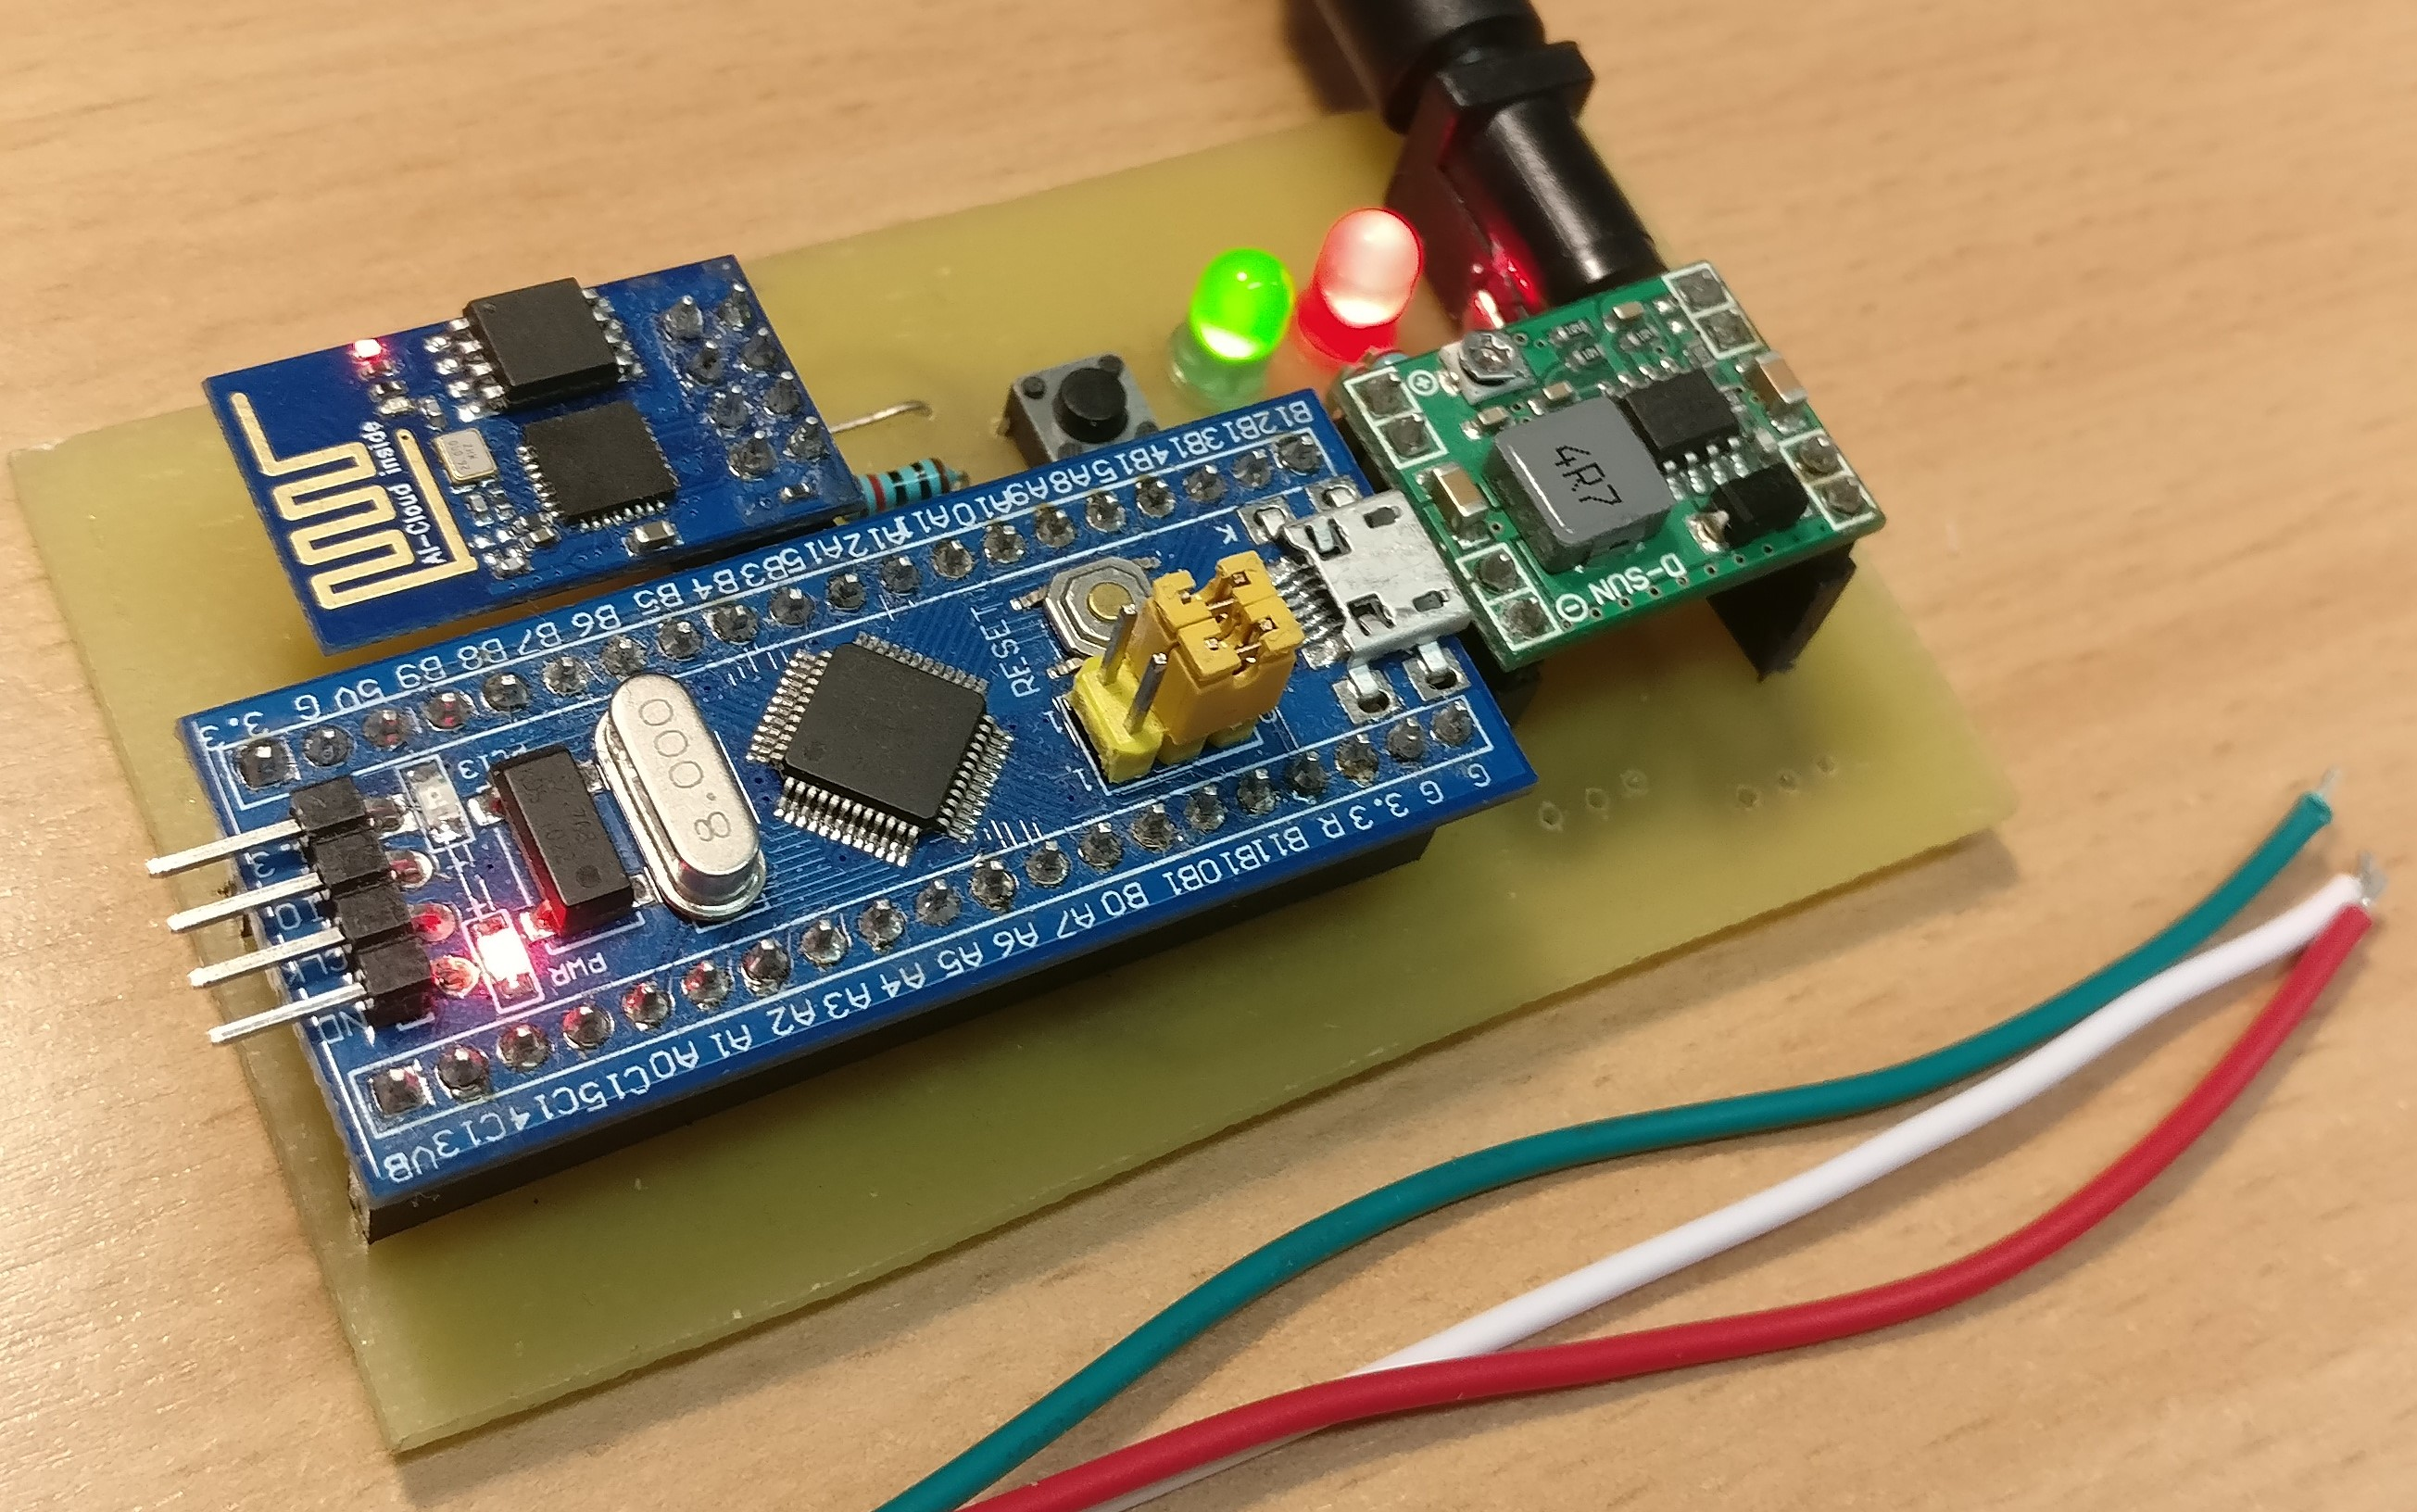
\includegraphics[width=6cm]{resources/pcb_res/pcb_v01.png}
            \caption{2. fázisú beforrasztott áramkör //TODO képet megcsinálni}
            \label{fig:pcb_v01}
        \end{figure}
        
        A 3. fázis tartalmazza DC/DC áramkör tervezését és mikrovezérlő perifériáival együtti integrálását egy nyomtatott áramköri lapra. 
        
        
        
 
 
        

v2 ugyon ugy modulokbol - csak vasalasos technikaval keszitett - mukodik de nem szep, illetve szeretnem emgtanulni a dc/dc tervezest - kepek\

v3 tervezes legyartas kinaban - kepek\\ 

    \subsection{Forrasztas}
forrasztas - hibajavitas\\
mit csinalnek mashogy legkozelebb\\

doboz tervezese fusionbe - kepek\\
3d nyomtatas - kepek\\
kesz termek - kepek\\

otthoni megvalositas, aramforraskereses, bekotes, zavarszüres ferritgyuruvel, teraszrol kepek\\

Beagyazott szoftver\\
Standard Peripheral Library (spl/stl ?) - a hatterben folyo folyamatok megertese miatt
interrupt, timer, uart, dma kezeles - mit miert
adatszerkezet
kommunikalas az espvel - bekonfiguralasa
ledsorral valo kommunikacio
effektek arduino neopixel librarybol 

\end{document}